%!TEX encoding = UTF-8 Unicode
\chapter{Aspekte}
Aspekte Aspekte
\section{Markt}
	\subsection{Markt für IT-Consulting}
	In den letzten Jahren ist der Markt für Beratungsleistungen in Deutschland stark gewachsen. Während im Jahr 1992 noch 5,9 Mrd.\texteuro Umsatz für Beratungsleistungen erzielt wurden(Quelle: BDU 2003), waren es im Jahr 2008 bereits 18,2 Mrd. \texteuro (Quelle:BDU 2009) und im Jahr 2012 betrug der Umsatz schon 22,30 Mrd. \texteuro (Abb.1).
\begin{figure}[htp]
\centering
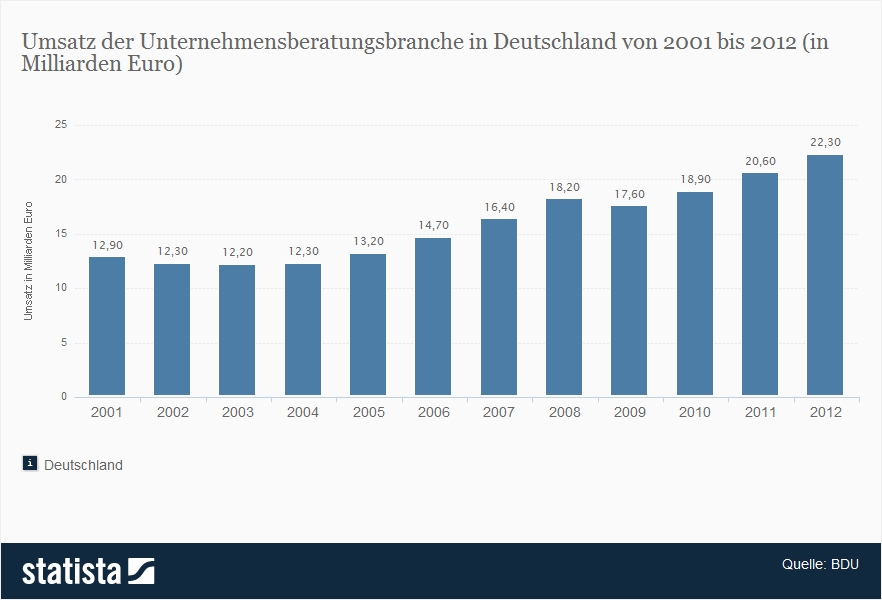
\includegraphics[width=0.7\linewidth]{./images/umsatz-der-unternehmensberatungsbranche-in-deutschland}
\caption{Umsatz der Unternehmensberatungsbranche in Deutschland}
\label{fig:umsatz_UBer}
\end{figure}


\section{Arbeitskultur}
	\subsection{Einleitung Arbeitskultur}
Arbeitskultur ist ....
Arbeitskultur ist eine Teilmenge der Kultur(Sitten,Bräuche) einer Nation. Sie gehört zum Beratungsprozess und spielt dabei nicht die unwesentlichste Rolle. IT-Consultans kennen innerhalb der wenigsten Zeit sehr viele Firmen und deren Mitarbeiter kennen. Berater arbeiten öfter durch Iteration mit Menschen:\\
1)aus unterschiedlichen Unternehmensebenen, angefangen von normalen Mitarbeiter(Interaktion mit Beratern während den Schulungsmaßnahmen bei IT-Neueinführung) bis zu Top-Managementebenen(Interaktion mit Beratern während der strategischen Fragen wie Planung von Anwendungssoftware, Analyse von Geschäftsprozessen usw.)\\

2)aus verschiedenen Branchen wie Finanzdienstleistung,Fahrzeugbau, Großhandel usw.
\begin{figure}[htp]
\centering
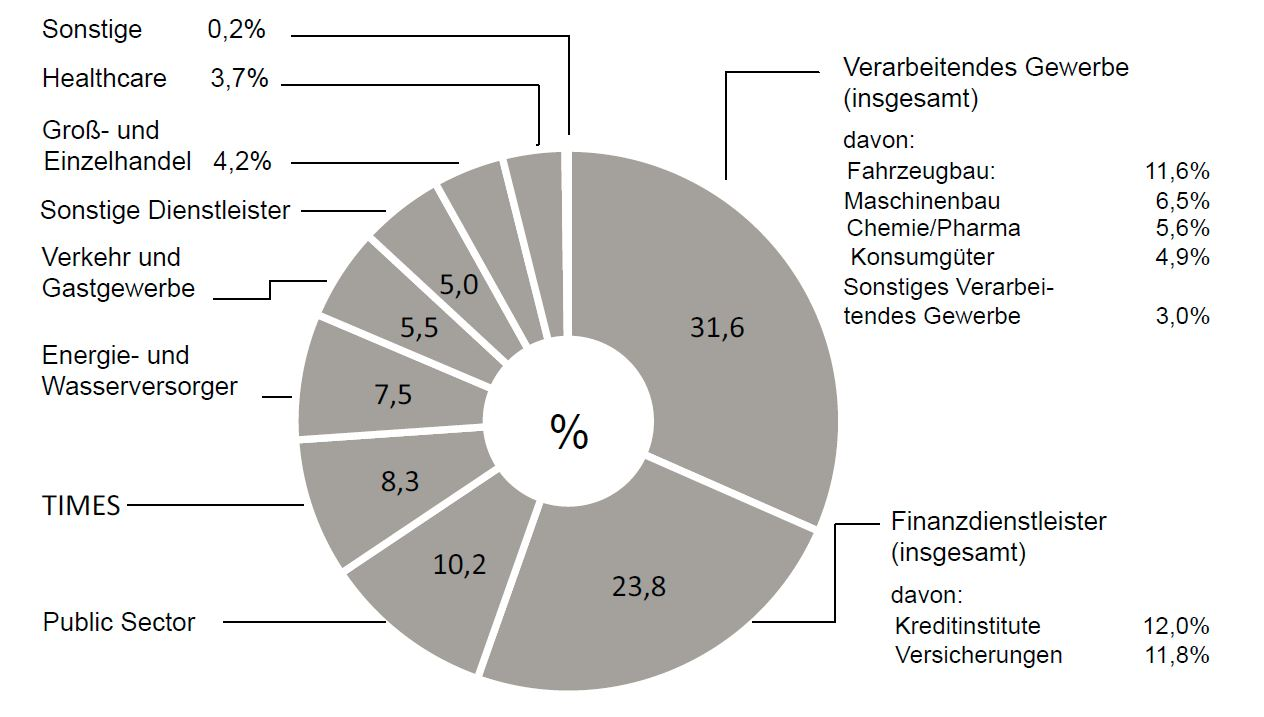
\includegraphics[width=10 cm]{./images/Auft_U_Beratung}
\caption{Aufteilung Unternehmensberatungen nach Branchen}
\label{fig:AufteilungUnternehmensberatung}
\end{figure}

3) aus unterschiedlichen Länder mit jeweils eigenartigen Kulturen.\\
 In diesem Punkt werden 2 Standardfälle erläutert um die Bedeutung der Arbeitskultur im Beratungsprozess zu zeigen.\\
 a) Das erste Fall ist ein IT-Consulting Unternehmen mit Beratern die aus unterschiedlichen Ländern kommen, die unterschiedliche Sprache sprechen und sich kulturell enorm unterscheiden.Diese Berater arbeiten zielgerichtet und ständig im Team. In diesem Fall wird dem Author dieser Arbeit sehr interessant inwieweit sich kulturelle Unterschiede auf das gemeinsame Ziel des Beratungsprozesses bei der Softwareeinführung auswirken können. Auch interessant ist hier wie die IT-Berater aus unterschiedlichen Länder mit Kunden aus Deutschland umgehen, ob die kulturelle Unterschiede einen Einfluss auf Kundenbeziehungen haben oder nicht. \\
 b) Das 2. Fall bezieht sich auf ein deutsches Unternehmen, das sich international agiert und Kunden aus unterschiedlichen Länder betreut. In diesem Fall müssen sich deutsche Mitarbeiter auf unterschiedliche Arbeitskulturen anpassen. Denn ein Meeting während des Mittagsessen in Japan ist widersinnig und wirkt unseriös, in USA dagegen ist es nicht ungewöhnlich, dass beim Essen wichtige Entscheidungen kollaborativ getroffen werden.  \\
Wegen der zeitlichen sowie thematischen Begrenzung liegt der Autor dieser Arbeit den Fokus nicht auf die Differenzierung dieser zwei Fälle sowie kulturelle Unterschiede der Berater, sondern nur auf die unterschiedliche Arbeitskulturaspekte, die für den Beratungsprozess ausschlaggebend sind. Teilaspekte der Arbeitskultur, die den Autoren dieser Arbeit interessant erscheinen, werden in folgenden Kapiteln vorgestellt und verglichen. In diesem Sinne werden diese 2. Fälle nicht weiterhin detaillierter behandelt.

\subsection{Einleitung in das Wesen des IT-Consultings}	

IT-Consulting ist eine wichtige Art des Consultings in IT-Fragen eines Unternehmens.Das Wesen des Consultings besteht im Allgemeinen darin, Unternehmen bei der Neustrukturierung des Anwendungslandschaften oder bei der Pflegung der bestehenden Informationssysteme zu unterstützen. Während des gesamten Beratungsprozesses bleibt Berater als externe Experte solange im Unternehmen bis die Probleme,die er mit seinem technischen Fachwissen zu lösen hat,nicht mehr existieren oder selbständig von den Mitarbeitern des Unternehmens gelöst werden können.
Um den Beratungsprozess zu verdeutlichen wird jetzt ein Beispielprozess aus der Praxis der IT-Beratung beschrieben. Ein Online-Handelsnternehmen möchte ein BI Standardsoftware einführen um die Daten für Analysezwecke aus dem ERP-System zu laden,um die potentiellen Kündiger zu vermeiden oder neue Kunden zu gewinnen.Am Anfang jedes Prozesses muss dem Berater die Organisationsstruktur des Unternehmens klar sein, um eine passende Lösung zu finden. Im Beratungsprozess gibt es eine Standardsoftware um IT-Problem zu lösen. Es gibt aber keine Standardlösung die für alle Unternehmensstrukturen passend ist,weil die Unternehmensstrukturen sehr unterschiedlich sind. Man beginnt die Verhandlung zwischen Unternehmensführung und den Beratern, die den Auftrag bekommen, indem man Vertrag abschließt. Danach beginnt die Analysephase. Hier wird die Unternehmensstruktur des Online-Handelsunternehmen auseinandergenommen, bis man erkennt wo die Software eingesetzt wird, Stellen wo die Reibungen entstehen werden,welche Ressourcen stehen zur Verfügung und welches Informationssystem sich am besten dafür eignet.
Es muss immer ein Feedback zwischen dem Berater und Unternehmensführer möglich sein.
nach der Analysephase beginnt die Umsetzungsphase indem eine neue IT-Architektur aufgebaut wird oder die vorhandene ergänzt wird.Im unseren Besipiel wird die ERP-Lösung mit dem BI Lösung erweitert, die vorhandene Architektur bleibt erhalten. In dieser Phase können auch die andere Berater aufgerufen werden, falls es viele komplizierte Realisierungsmaßnahmen gibt.
Nachdem die Informationssystem erfolgreich installiert ist, beginnen die Schulungsmaßnahmen, damit die Mitarbeiter des Unternehmen in der Lage sind mit diesem System umgehen zu können. Zum Schluss kommt die Wartungsphase und Intensität der Beratungsdienstleistung nimmt langsam ab. 
	\subsection{Bedeutung der Arbeitskultur für IT-Consulting}
In wie weit ist es wichtig Arbeitskultur für den Beratungsprozess zu betrachten? Anhand vom unseren Beispiel ist es zu erkennen dass die Berater in jeder Phase der Softwareeinführung mit den Unternehmensvertretern kommunizieren sollen. Es ist wichtig,dass die Berater genug technisches Know-how mitbringen, noch wichtiger sind die Soft Skills, die für erfolgreiche Geschäftsbeziehungen entscheidend sind.``IT Business is People's Business. Diese Leitlinie impliziert, dass der Erfolg von IT-Projekten maßgeblich von der Kompetenz des Beraters abhängt.´´
%(Quelle: http://www.it-production.com/index.php?seite=einzel_artikel_ansicht&id=26189)
 Welche Social Skills des IT-Beraters sind für Deutscher als obligatorisch herausgestuft? Sind diese persönlichen Eigenschaften auch für die anderen Nationen von der Bedeutung? Unternehmensführung und IT-Berater müssen bei der Lösung des Problems einig werden. Der Berater muss Unternehmen für seine vorgeschlagene Lösung überzeugen. Muss man, um dies zu realisieren, nur eine gute Software anbieten und als vertrauenswürdiges Unternehmen am Markt agieren oder reichen diese Bedingungen beispielsweise in Indien nicht aus ,weil der Berater aus anderer Kaste ist.Denn die Kastenzugehörigkeit hat in Indien bis heute kulturelle und soziale Auswirkungen auf viele Lebensbereiche. % (Quelle: http://www2.klett.de/sixcms/list.php?page=geo_infothek&miniinfothek=&node=Indien&article=Infoblatt+Kastensystem+in+Indien)
 Für diese Arbeit ist wichtig zu wissen wie die Arbeitskultur in ausgewählten Länder sich unterscheidet und in wie weit diese den Beratungsprozess beeinflussen kann.
 
%Sind überhaupt Softs Skills entscheidend für einige Länder oder spielt eher die technische Ausrüstung des Beraters bedeutsame Rolle. Schwerpunkte:\\ 1)Für die Autoren dieser Arbeit ist es aus persönlichen Interessen wichtig zu wissen wie man Unternehmen aus anderen Ländern berät und indem man als Berater ins Ausland geschickt wird.\\2)Wie verläuft der Beratungsprozess in einigen Länder die bedeutungsvoll und potenzialreich für IT-Consulting sind.



In den folgenden Kapiteln wird Arbeitskultur von ausgewählten Länder(Russland, USA, Deutschland usw.) untersucht und zum Schluss werden einige interessante Fakten verglichen und diskutiert. 

\subsection{Teilaspekte der Arbeitskultur und ausgewählte Länder}
Hier werden Aspekte aufgelistet die für Arbeitskultur von der Bedeutung sind (Arbeitsplatz, Mitarbeiterverhältnisse,Hierarchien,Organisation,Lebensunmstände etc).
Autoren dieser Arbeit haben sich einige Teilaspekte der Arbeitskultur sowie die zugehörigen Länder durch Brainstorming überlegt. Dazu wird übersichtshalber eine Matrix aufgestellt. Felder dieser Tabelle bleiben zuerst leer und nach dem die einzelne Aspekte von den Ländern recherchiert und vorgestellt werden, wird die Matrix noch mal mit den ausgearbeiteten Feldern ausgefüllt. damit kann man auch die Rechercheergebnisse testen, ob sie erfolgreich waren oder nicht. \\
\\
\begin{table}[htp]
\begin{tabular}{|c|c|c|c|c|c|c|}
\hline  Aspekt/Land& Deutschland & USA & Russland & Japan & Indien & Brasilien \\ 
\hline Hierarchien  & ? & ? & ? & ? & ? & ? \\ 
\hline  Kundenverhältnisse& ? & ? & ? & ? & ? & ? \\ 
\hline  spezielle Rechtslage& ? & ? & ? & ? & ? & ? \\ 
\hline  Grad des intuitiven Handelns& ? & ? & ? & ? & ? & ? \\ 
\hline  Kritikfähigkeit& ? & ? & ? & ? & ? & ? \\ 
\hline  Tagesrythmus& ? & ? & ? & ? & ? & ? \\ 
\hline  Organisation& ? & ? & ? & ? & ? & ? \\ 
\hline  Lebensumstände& ? & ? & ? & ? & ? & ? \\ 
\hline  Zeitmanagement& ? & ? & ? & ? & ? & ? \\ 
\hline  Work-Life-Balance& ? & ? & ? & ? & ? & ? \\ 
\hline 
\end{tabular} 
\caption{Matrix der Arbeitskultur, Quelle: eigene Darstellung xD}
\end{table}


	\subsection{Russland}
	% was mache ich mit den Quellen in original Sprache?-genau so wie de 
	Russland ist ein Wachstumsmarkt mit Zukunft. Heute ist der damals geschützter russischer Markt offen für Exporte und Investitionen aus Deutschland.Dies gilt sowohl für IT-Beratungs Unternehmen, die ihre Softwareprodukte in Russland integrieren auch für russische Manager, die bei der Informationstechnologie auf westliches Know-how setzen.\\
	%(Quelle: http://www.it-production.com/index.php?seite=einzel_artikel_ansicht&id=26189)
	Da der Markt für IT-Beratung neu ist, muss man als IT-Berater aus Westen ganz viele Entscheidungen intuitiv treffen. Hier weden natürlich die Soft Skills gefragt. Technische Fähigkeiten, funktionales Wissen und Branchen-Know-how sind selbstverständlich vorausgesetzt. Sonst wären die höheren Tarife für westlichen Berater ungerechtfertigt. Mit anderen Wörtern müssen die deutschen Beratern mit ihrem Wissen auf einer Stufe höher stehen als russischen Kollegen, damit sie für russische Softwareprojekte eingesetzt werden können. 
	Der russischer Senior-Consultant aus Moskau verdient im Mittel 3845 € im Jahr. Das ist für russische Verhältnisse relativ hoher Gehalt. Doch gibt es in Russland sehr starke regionale Gehaltsunterschiede. Aus dem unten stehenden Diagramm kann man den Unterschied des monatlichen 
	Gehalts für SAP-Berater ermitteln. Im Großen und Ganzen verdient man in beiden Metropolen Moskau und Sankt-Petersburg ca. das doppelte wie in anderen Großstädten wie Rostov, Wolgograd oder Omsk.
	\\
\begin{figure}[htp]
\centering
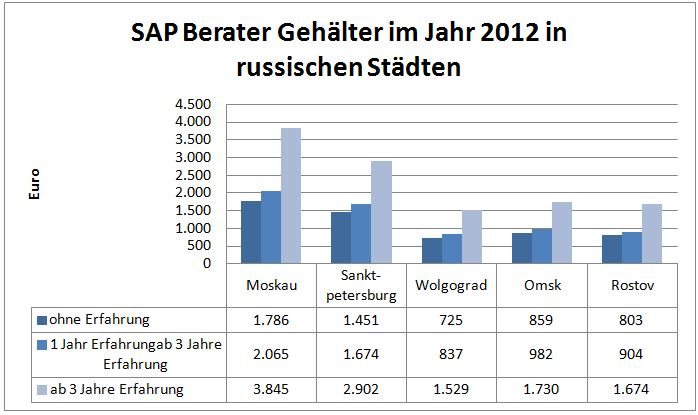
\includegraphics[width=0.7\linewidth]{./images/SAP-Berater_Gehalt_RU}
\caption{SAP-Berater Gehälter in Russland}
\label{fig:SAP-Berater_Gehalt_RU}
\end{figure}

	
	%Quelle:http://www.tadviser.ru/index.php/\CYRS\cyrt\cyra\cyrt\cyrsftsn\cyrya:\CYRR\cyrery\cyrn\cyro\cyrk_\cyrt\cyrr\cyru\cyrd\cyra_\cyrv_\CYRR\cyro\cyrs\cyrs\cyri\cyri_\CYRI\CYRT_\cyri_\cyrt\cyre\cyrl\cyre\cyrk\cyro\cyrm
	


	Senior IT-Berater aus Deutschland verdient im Mittel 6.250 € im Monat. Die deutschen Berater, die nach Ausland geschickt werden, haben noch höheren Gehaltstarife. %(Quelle: http://www.computerwoche.de/a/sap-berater-90-000-euro-nach-fuenf-jahren,2535266)
	Der Junior Berater im IT Umfeld ohne Projekterfahrung  verdient in Russland ca. 1200 € monatlich.
	Sein deutscher Kollege mit den gleichen Qualifikation und Erfahrung verdient ca. drei mal so viel (3750 €).
	%Quelle:http://www.computerwoche.de/a/sap-berater-90-000-euro-nach-fuenf-jahren,2535266
	\\
	\\
	´´Der Zerfall der Sowjetunion und die Reformen im wirtschaftlichen und sozialen Gefüge Russlands haben einen erheblichen Einfluss auf die Arbeitskultur in gegenwärtigen russischen Organisationen´´. Deswegen überlappen sich die kulturelle mit reformbedingten Faktoren der Arbeitskultur. Autor dieser Arbeit möchte eher auf Beschreibung von Teilaspekten  eingehen und nicht auf die Erklärungen der Tatsache. Ursachen.\\%Quelle http://joconsult.netzmerk.com/pup/prozess-de.pdf
	
	%	\textbf{Aspekt Arbeitsplatz}\\``Der Arbeitsplatz ist für viele russische Arbeitnehmer nicht nur der Ort, an dem das Einkommen erarbeitet wird, er hat auch eine große soziale Bedeutung: Familienangehörige von Kollegen kennen sich untereinander, wenn der Kindergarten geschlossen hat, bringen Frauen ihre Kinder mit zur Arbeit etc. Eine Abgrenzung zwischen Berufstätigkeit und Arbeitsleben, wie sie im westeuropäischen Sinne üblich ist, wird nicht vorgenommen.``-> Wie kann die Aussage den Beratungsprozess beeinflussen?\\
	\textbf{Team und Organisation: Russischer Arbeitskollektiv gegen westlichen Team}\\
	``Das Arbeitskollektiv wurde in der sowjetischen 
	Epoche als das zentrale soziale Handlungsfeld propagiert und die Geschlossenheit der Gruppe ist wichtiger als die Selbstverwirklichung des Einzelnen Gruppenmitglieder.`` Gruppeninterne Konflikte wurden deshalb vermieden oder nicht diskutiert. Der Unterschied gegen dem westlichen Team besteht darin, dass russischer Kollektiv eine dauerhafte Einrichtung ist klar zugewiesene Leitungskompetenzen, die vom Vorgesetzten ausgeübt werden, während das Team nur für die Dauer eines bestimmten Projektes eingerichtet wird und sich durch die Gleichberechtigung aller Teammitglieder auszeichnet.Quelle:
	So ein Kollektiv für Beratungszwecke ist demzufolge nicht flexibel und ist zu stark weisungsgebunden. Die Aufgaben im Kollektiv werden vom Vorgesetzten vorgeschrieben, im unser Fall von einem Projektleiter oder einem Manager. Solche Führungspersonen sind im IT-Beratungsfall an einen Office gebunden und sind immer im Office während die Berater immer unterwegs bei den Kunden sind. Daher müssen die Entscheidungen immer intuitiv und unabhängig von dem Vorgesetzten getroffen werden. Das ist eine Widerspiegelung dem Prinzip des russischen Kollektivs. ``Russische Organisationen zeichnen sich durch eine Konzentration von Macht auf die Führungskräfte aus. Ohne den ``Natschalnik`` werden keine Entscheidungen getroffen.`` %Quelle http://joconsult.netzmerk.com/pup/prozess-de.pdf
	Verlagerung von Entscheidungen auf die Mitarbeiter wird in Russland selten stattfinden,deswegen werden die Mitarbeiter von der Verantwortung befreit und übernehmen oft nur Anweisungsfunktionen. Für  den Beratungsprozess ist diese Tatsache ein reisen Minuspunkt, weil die Berater das interdisziplinäres Wissen besitzen und  den vollen Handlungsspielraum in der IT-Beratungsszene brauchen.
	Zu erwähnen wäre noch, dass die jungen Menschen von solcher Stereotypen weiter entfernt sind als die ältere ``sowjetische`` Generation. \\

	\textbf{Personalauswahl und Gesetze}\\
	 Eine weitere wichtige Besonderheit ist die Personalauswahl. Häufig erfolgt die Auswahl von neuen 
	 Mitarbeitern nicht nach Kriterien der fachlichen Kompetenz. Oft werden Arbeitsplätze unter Verwandten und 
	 Freunden vergeben. Es existieren fast keine etablierten Mechanismen von Angebot und Nachfrage auf dem 
	 Arbeitsmarkt. Vakanzen werden häufig nicht an den fachlich geeignetsten Bewerber vergeben, sondern an 
	 ``unseren Mann``(nash celovek).\\
	 Ein weiteres für Russland typisches Merkmal ist, dass Gesetze, Bestimmungen und 
	 Regelungen keinen eindeutig verbindlichen Charakter haben. In Abhängigkeit von der 
	 Situation und den involvierten Personen, können Regeln oder Gesetze bewusst 
	 unberücksichtigt bleiben. Wie sich jedoch diese Abstufung darstellt ist nicht vorhersagbar. Das liegt auch daran, dass das russische Volk und die russischen Behörde sich einander nicht zutrauen.
	 %Quelle http://joconsult.netzmerk.com/pup/prozess-de.pdf
	 
	 \textbf{Arbeitszeit und Urlaub}\\
	 Die gesetzliche Wochenarbeitszeit in Russland beträgt 40 Stunden. Doch in meisten Fällen wird diese Grenze total überschritten. Die IT-Spezialisten arbeiten zwischen 10 und 11 Stunden am Tag in einem 5 Tage-Rhythmus. Oft wird auch 6- Tage- Woche praktiziert. Die deutschen Berater arbeiten ca. 10 Stunden  im 4 Tage-Rhythmus und sind direkt beim Kunde vor Ort. Am Freitag gibt es entweder Zeit für eigene Weiterbildung im Home-Office oder ein lokales Meeting in der Firma bis nachmittags.
	 In vielen Tarifverträgen in Deutschland beträgt der Jahresurlaub 30 Arbeitstage. In Russland sind es dagegen nur 24 Tage. Der Arbeitstag beginnt bei russischen nicht produzierenden Firmen um 9 oder 10 Uhr. Wenn ein IT-Berater um 10 Uhr mit seiner Arbeit beginnt, dann ist er um 20-21 Uhr zu hause. Natürlich bleiben viele Sachen zu hause liegen und es bleibt sehr wenig Zeit für privates Leben.  %Quelle: http://de.rusbiznews.com/about/PervyirazvRossii 
	 \\
	 
	 \textbf{Reisen und Pünktlichkeit}\\
	 IT-Berater Beruf ist eine Tätigkeit, die mit höheren Reisebereitschaft verbunden ist. In Deutschland sind die Berater oft mit Autos unterwegs. Von einem deutschen Großstadt bis zum anderen braucht man beispielsweise 4-5 Stunden.In Russland gibt es 2 grundsätzliche Transportprobleme mit dem Consulting-Hintergrund, die dem Autor auf den Ersten Blick erscheinen: Staus in Moskau und große Entfernungen zwischen den russischen Städten.Das Land ist nahezu unendlich groß und weit(es umfasst 11 Zeitzonen).
	 Zwischen Moskau und Nowosibirsk sind es ca 4 Stunden nur Flugzeit und plus 3 Stunden Zeitunterschied. Wenn ein Berater aus Moskau seinen Arbeitstag am Montag in Nowosibirsk beginnen möchte, muss er schon am Sonntag ausreißen. Die Reisen sind erschöpfend und werden von russischen Berater nicht so gern angenommen.\\
	 Laut dem russischen Rating mit dem Namen "Consulting research" aus 21 größten IT-Consulting-Unternehmen befinden sich 13 Unternehmen in Moskau.%Quelle: http://www.cfin.ru/consulting/rating_uni/it_consulting_2005.shtml 
	 Aus 100 größten russischen IT-Unternehmen befinden sich in Moskau 71 Firmen. 
	 %Quelle:http://www.cnews.ru/reviews/new/rynok_it_itogi_2012/review_table/1d5d1838fd010e16936649555e52b4dd1655219b/
	 Moskau ist nicht nur ein teuerster Hauptstadt der Welt und ein wirtschaftliches Zentrum des Landes, sondern auch ein strategisches Standort für IT geworden.
	 Mit der Stadtwachstum wachsen parallel die Staus.``Nach Angaben des GPS-Navigationsanbieters TomTom ist Mosaku Nummer eins unter den schlimmsten Stau-Städten der Welt.``%Quelle: http://de.ria.ru/society/20130405/265872844.html
	 Da die Berater öfters unterwegs sind, ist es eine große Anstrengung in Moskau Auto zu fahren. Um von A nach B zu kommen wird ganz oft ein Metro benutzt. 
	 Deswegen ist es in Moskau ``erlaubt`` dem Berater halbe Stunde zum Meeting oder zum  Kunde zu spät zu kommen. Allgemein sind die Russen nicht pünktlich, die Termine werden nicht immer eingehalten, E-Mails werden nicht sofort beantwortet und die Versprechungen sind nicht immer realistisch. Deswegen muss man als Berater diese Verzögerungen einplanen.%Quelle: http://www.sekretaria.de/rubrik_GR/geschrakt/Der_Russland-Knigge--A-2715.html
	  \\ 
	  \\
	 	 \textbf{Hierarchie}\\
	 Hierarchien und Entscheidungsfreudigkeit
	 Wenn Verhandlungen anstehen, sollten Sie beachten, dass Entscheidungen oft länger dauern. Mehrere Stellen müssen konsultiert werden bis die Entscheidung fällt. Die Hierarchien sind nicht immer klar erkennbar, dadurch laufen Sie Gefahr, Ihre Zeit in fruchtlosen Gesprächen zu verlieren. Es lohnt sich also noch vor Beginn der Verhandlungen herauszufinden, wer das entscheidende Wort hat.
	 %Quelle: http://www.sekretaria.de/rubrik_GR/geschrakt/Der_Russland-Knigge--A-2715.html
	 ``Flache Hierarchien und ``win-win`` sind nicht die Sache der Russen`` %Quelle:http://www.wissen.de/business-knigge-osteuropa
	 
	\subsection{China}
	
	
	\subsection{USA}
	
	
	\subsection{Deutschland}
	
	
	\subsection{Indien}


\section{Wissenschaft}